\documentclass{jmlr} % ML4H 2026 template base
\mlhtrack{proceedings}
\jmlrproceedings{ML4H}{Submitted to ML4H 2026: \mlhtrackname}

\usepackage{booktabs}
\usepackage{siunitx}
\usepackage{graphicx}
\usepackage{url}
\usepackage{hyperref}

\input{math_commands.tex}

\title{Calibration Transfer for Dominant-Cell-Type Reliability Scores in Spatial Transcriptomics Deconvolution}

\author{\Name{Anonymous Authors} \Email{anonymous@example.com} \\
      \addr Anonymous Institution}

\begin{document}

\maketitle

\begin{abstract}
Miscalibrated reliability scores in spatial transcriptomics deconvolution models poses a critical risk to downstream clinical discovery. We present a rigorously controlled benchmarking study evaluating reliability calibration under synthetic deployment-time shifts (binomial dropout and Poisson noise). Rather than identifying a universally optimal post-hoc calibrator, we demonstrate that calibrator robustness under shift is highly conditional on two factors: taxonomic granularity and model architecture. First, for fine-grained deconvolution, Isotonic Regression retains an absolute calibration advantage but degrades steeply under shift due to narrow support coverage of the fitted sparse marginals, presenting a severe relative stability concern compared to Temperature Scaling. Beta[a=b] calibration (a constrained variant of Kull et al., 2017) offers intermediate flexibility but similarly degrades. Second, while Temperature Scaling successfully rescues amortized models (e.g., DestVI), it fails on per-spot optimized models (e.g., \texttt{cell2location}) whose un-amortized posteriors become too severely skewed under shift for a single scalar parameter to adequately flatten without collapsing to uniform---for these, Isotonic Regression is preferable. By contrast, for coarse-grained tasks, broad support coverage prevents Isotonic density-shift degradation while Temperature Scaling becomes overly restrictive, degrading DestVI outright and only partially correcting \texttt{cell2location}. Using a five seeded repeated holdout replicates pipeline with 500 bootstrap resamples, our results indicate that method choice should dynamically match the model architecture and taxonomic resolution of the spatial problem.
\end{abstract}

\paragraph*{Keywords}
Spatial Transcriptomics, Confidence Calibration, Variational Inference, Distribution Shift

\section{Data Availability}
As detailed in the front matter, raw data utilized in this study are publicly accessible via standard repositories (scRNA-seq Mouse Cortex reference: \texttt{scvi-tools} tutorials; scRNA-seq DropViz Hippocampus reference: DropViz portal; Visium: 10x Genomics Datasets \textit{V1\_Mouse\_Lymph\_Node}; Slide-seqV2: Broad Institute Single Cell Portal \textit{SCP815}), and our fully reproducible pipeline is provided at \url{https://anonymous.4open.science/r/transcriptomics-AF35/}.

\paragraph*{Institutional Review Board (IRB) and Ethics}
IRB review is not applicable because this study uses only publicly available animal-derived datasets and involves no human participants. No new animal experimentation was performed.

\section{Introduction}
\label{sec:intro}
Spatial transcriptomics models face persistent challenges in standardization and scalability. A critical failure mode is miscalibrated confidence in clinical deconvolution pipelines. Existing benchmarks, such as the comprehensive Spotless pipeline \citep{sang2024spotless}, rigorously evaluate point-estimate accuracy across methods and dozens of silver standards, but few focus specifically on whether models \textit{know when they are wrong}. 

Crucially, downstream biological and clinical discovery is sensitive to these miscalibrations. For instance, in tumor microenvironment characterization, if a spatial model confidently but incorrectly predicts an immunosuppressive cell type as the dominant population in a tumor region, it could lead to improper patient stratification for immunotherapies. Ensuring models are correctly calibrated under technical shifts is a prerequisite for clinical deployment, before these tools can safely inform high-stakes diagnostic or therapeutic decisions. Note that our quantitative evaluation in this work focuses exclusively on murine cortex datasets as an initial validation domain.

In this paper, we focus on the calibration of spatial deconvolution models, specifically evaluating DestVI \citep{lopez2022destvi} and \texttt{cell2location} \citep{kleshchevnikov2022cell2location}, under controlled deployment-time shifts. This work represents a comprehensive evaluation intended to establish a rigorous baseline---featuring a fully reproducible pipeline, genuine train/calibration/test splits held constant under shift, and paired significance testing---and validation on authentic biological spatial datasets.

\section{Related Work}
\label{sec:related}
Reliability score calibration of modern neural networks was formalized by \citet{guo2017calibration}, demonstrating that deep models often exhibit severe overconfidence but can be realigned using post-hoc methods like temperature scaling or isotonic regression. Subsequent work by \citet{ovadia2019can} established that model calibration frequently degrades under dataset shifts. We extend these foundational frameworks to spatial transcriptomics, where such rigorous evaluations are scarce despite widespread distribution shifts between platforms. Note that standard fixed-bin ECE estimators can be statistically biased \citep{roelofs2022mitigating}, which remains a general caveat for these absolute calibration magnitudes. Prior work has investigated calibrated uncertainty for spatial gene-expression prediction \citep{sun2024tissue}, and hierarchical cell-type taxonomies via conformal prediction sets \citep{corbetta2024conformal}, but these approaches focus on optimizing point-estimate metrics or set-valued bounds rather than directly addressing point-wise probabilistic confidence for clinical interpretation. Recent methods such as ReliST \citep{relist2026} have provided a post-hoc, model-agnostic risk layer that preserves base predictions and has been evaluated across multiple organs and models. In this work, we take a complementary approach: instead of developing a novel risk score, we comprehensively evaluate standard probabilistic calibration methods (Temperature Scaling and Isotonic Regression) applied post-hoc to compositional outputs under controlled technical distribution shift. While advanced deconvolution models like LETSmix \citep{zhan2025letsmix} and HarmoDecon \citep{wang2025harmodecon} offer robust architectural improvements for handling technical noise, they do not guarantee reliable confidence bounds out-of-the-box. We diverge from these architecture-centric approaches by providing a rigorous empirical audit of how standard calibration heuristics (Temperature Scaling and Isotonic Regression) perform under the deployment-time technical shifts (e.g., cross-platform noise and dropout) uniquely characteristic of spatial transcriptomics.

\section{Materials and methods}
\label{sec:methods}
\subsection{Synthetic Datasets and Evaluation}
We benchmarked the variational inference models DestVI and \texttt{cell2location} on mouse cortex pseudo-spots. We evaluated calibration using Expected Calibration Error (ECE) for the discrete classification task of predicting the dominant (highest proportion) cell type within a spot. Finally, we evaluated the full continuous compositional output using Compositional Root Mean Square Error (RMSE).

\subsection{Training, Calibration, and Test Composition}
To establish ground-truth for ECE computation, for each of the $n=5$ computational folds, we randomly split the source single-cell data into two completely disjoint pools. The CondSCVI reference prior was trained exclusively on the 50\% source-cell training pool. From the disjoint 50\% source-cell test pool, we generated a fresh set of pseudo-spots. These pseudo-spots were rigorously partitioned into three disjoint splits: 50\% training, 25\% calibration, and 25\% test, confirming no train/test leakage and no leave-one-out methodologies. Exactly one DestVI model was trained to convergence exclusively on the clean training split. Temperature Scaling and Isotonic Regression were fit exactly once, using the frozen model's predictions on the clean calibration split. Under this design, within-replicate independence is guaranteed; across-replicate independence is not, given the finite shared source-cell pool, meaning $p$-values are indicative rather than exact. We utilized $n=5$ rather than $n=10$ computational folds to accommodate the linear increase in compute memory required for our expanded shift-type sweeps.

\subsection{Deployment-Time Shift Simulation}
To simulate synthetic capture-efficiency shift motivated by cross-platform variability, we synthetically downsampled the read counts of the held-out test split via a binomial dropout process \citep{townes2019feature}. We also evaluated ambient Poisson noise injection to ensure robustness across diverse technical shift artifacts.

\subsection{Calibration and Auxiliary Metrics}
Isotonic Regression is a non-parametric method that learns a monotonically increasing step-function to map uncalibrated confidences to empirical correctness probabilities. Because it can learn an arbitrary number of knots, it is theoretically optimal given infinite data but heavily prone to overfitting finite bins. 

As a structural intermediate, we also evaluate Beta Calibration \citep{kull2017beta}, a two-parameter parametric mapping applied via logistic regression on the log-odds of the predicted confidences. This serves to directly test the ``single-parameter versus non-parametric'' flexibility spectrum.

Note that for compositional spatial vectors, we define the confidence as the maximum predicted proportion (the argmax). This reduction is standard because the primary downstream task is typically discrete class assignment (i.e., assigning a spot to its dominant cell-type niche). Therefore, we prioritize calibrating the maximum predicted probability rather than full posterior credible intervals.

Expected Calibration Error (ECE) approximates the expected difference between confidence and true accuracy by partitioning predictions into $M=10$ equal-width bins. We also compute Adaptive-binning ECE \citep{nixon2019measuring}, which ensures equal sample sizes per bin, and Negative Log-Likelihood (NLL) as auxiliary metrics (Appendix B). For evaluation, confidence intervals are derived from 500 bootstrap resamples of the test set per cross-validation fold, though we note that for the $k=4$ classification with 5 folds, the discrete combinations inherently limit statistical power to a combinatorics quantization minimum of $1/C(9,4) = 1/126$.

\section{Results}
\label{sec:results}
\subsection{Calibration under Synthetic Shift}
As shown in Table \ref{tab:results}, the baseline uncalibrated DestVI model exhibited severe overconfidence, achieving an uncalibrated ECE of $0.215$ on clean source data. As binomial dropout was introduced to simulate progressive technical efficiency loss, the baseline ECE degraded monotonically, reaching $0.259$ under severe 80\% dropout.

Across all technical shift conditions, Isotonic Regression achieved a strictly lower absolute ECE than Temperature Scaling. However, a deeper examination of the degradation rates reveals a severe relative stability concern, pointing to a potential crossover beyond the tested range. Table~\ref{tab:results} shows a consistent absolute advantage for Isotonic Regression alongside a divergence in degradation rates. In the unshifted domain ($0\%$ dropout), both Temperature Scaling and Isotonic Regression successfully correct the uncalibrated baseline ($0.215 \pm 0.007$), achieving respective ECEs of $0.067 \pm 0.004$ and $0.010 \pm 0.003$. However, as technical noise (capture efficiency dropout) strictly increases, the non-parametric Isotonic mapping degrades nearly three times faster than Temperature Scaling. A paired t-test across the 5 computational folds comparing the change in ECE ($\Delta \text{ECE}$) between shifted and clean conditions confirms that this differential degradation rate is statistically significant ($p = 0.024$, evaluated on DestVI under 80\% dropout). Under $80\%$ dropout, Isotonic Regression's ECE more than doubles to $0.028 \pm 0.004$, while Temperature Scaling remains structurally stable at $0.069 \pm 0.005$. The two-parameter Beta Calibration model exhibited similar degradation to Isotonic Regression, suggesting that even limited parametric flexibility is vulnerable to these shifts (Appendix B).

Interestingly, while Isotonic Regression achieves a massive numerical ECE advantage, it fails to substantially improve the continuous Brier Score over Temperature Scaling (e.g., $0.031$ vs.\ $0.036$ at baseline, a minimal gain compared to the massive ECE drop). This divergence, paired with NLL worsening significantly for Isotonic mappings, strongly suggests that Isotonic Regression is overfitting to binning artifacts to artificially minimize ECE, rather than fundamentally improving the continuous probability manifold \citep{roelofs2022mitigating, kumar2019calibration}. Furthermore, the theoretical expected ECE noise floor for a perfectly calibrated model with $N=500$ test spots (computed under a uniform Dirichlet reference distribution) is approximately $0.021$ for a 23-class problem and $0.041$ for a 4-class problem. Isotonic Regression's reported ECEs of $0.010$ ($k=23$) and $0.011$ ($k=4$) fall significantly below these theoretical minimums (noting that an estimator whose output collapses into few bins naturally admits a lower noise floor than the reference simulation). This is consistent with the hypothesis that its non-parametric mapping artificially deflates ECE by collapsing predictions into fewer, heavily-populated bins where finite-sample noise is minimized.

\begin{table*}[t!]
\centering
\footnotesize
\caption{Synthetic benchmark calibration results for DestVI across progressive technical domain shifts (binomial capture efficiency dropout and ambient Poisson noise injection). Results shown are mean ECE / Brier, with 95\% confidence intervals derived from 500 bootstrap resamples of the test-set predictions within each computational fold. No bootstrap CI is reported for the uncalibrated column because it is a fold-level mean.}
\label{tab:results}
\begin{tabular}{l c c c c}
\toprule
Shift & Uncalibrated & Temp Scaled (95\% CI) & Isotonic Reg (95\% CI) \\
\midrule
0\% Dropout (1.0, baseline) & ECE: 0.215 & 0.067 [0.045, 0.081] & 0.010 [0.003, 0.016] \\
                            & Brier: 0.200 & 0.036 [0.022, 0.051] & 0.031 [0.014, 0.049] & \\
20\% Dropout (0.8) & ECE: 0.220 & 0.068 [0.046, 0.082] & 0.010 [0.002, 0.019] \\
                   & Brier: 0.205 & 0.037 [0.022, 0.052] & 0.032 [0.014, 0.050] & \\
40\% Dropout (0.6) & ECE: 0.228 & 0.070 [0.047, 0.084] & 0.011 [0.003, 0.021] \\
                   & Brier: 0.213 & 0.038 [0.023, 0.051] & 0.032 [0.015, 0.049] & \\
60\% Dropout (0.4) & ECE: 0.238 & 0.070 [0.052, 0.082] & 0.016 [0.007, 0.025] \\
                   & Brier: 0.222 & 0.039 [0.027, 0.051] & 0.034 [0.019, 0.048] & \\
80\% Dropout (0.2) & ECE: 0.259 & 0.069 [0.052, 0.085] & 0.028 [0.011, 0.048] \\
                   & Brier: 0.243 & 0.042 [0.031, 0.050] & 0.036 [0.022, 0.046] & \\
\midrule
Poisson Noise ($0.5\times$) & ECE: 0.207 & 0.067 [0.061, 0.074] & 0.012 [0.004, 0.020] \\
                            & Brier: 0.198 & 0.037 [0.021, 0.051] & 0.033 [0.015, 0.050] & \\
Poisson Noise ($1.0\times$) & ECE: 0.198 & 0.068 [0.064, 0.072] & 0.013 [0.005, 0.022] \\
                            & Brier: 0.190 & 0.037 [0.021, 0.052] & 0.034 [0.016, 0.050] & \\
Poisson Noise ($2.0\times$) & ECE: 0.176 & 0.054 [0.034, 0.066] & 0.016 [0.007, 0.028] \\
                            & Brier: 0.170 & 0.036 [0.020, 0.057] & 0.034 [0.015, 0.056] & \\
\bottomrule
\end{tabular}
\end{table*}


\begin{figure}[htbp]
\centering
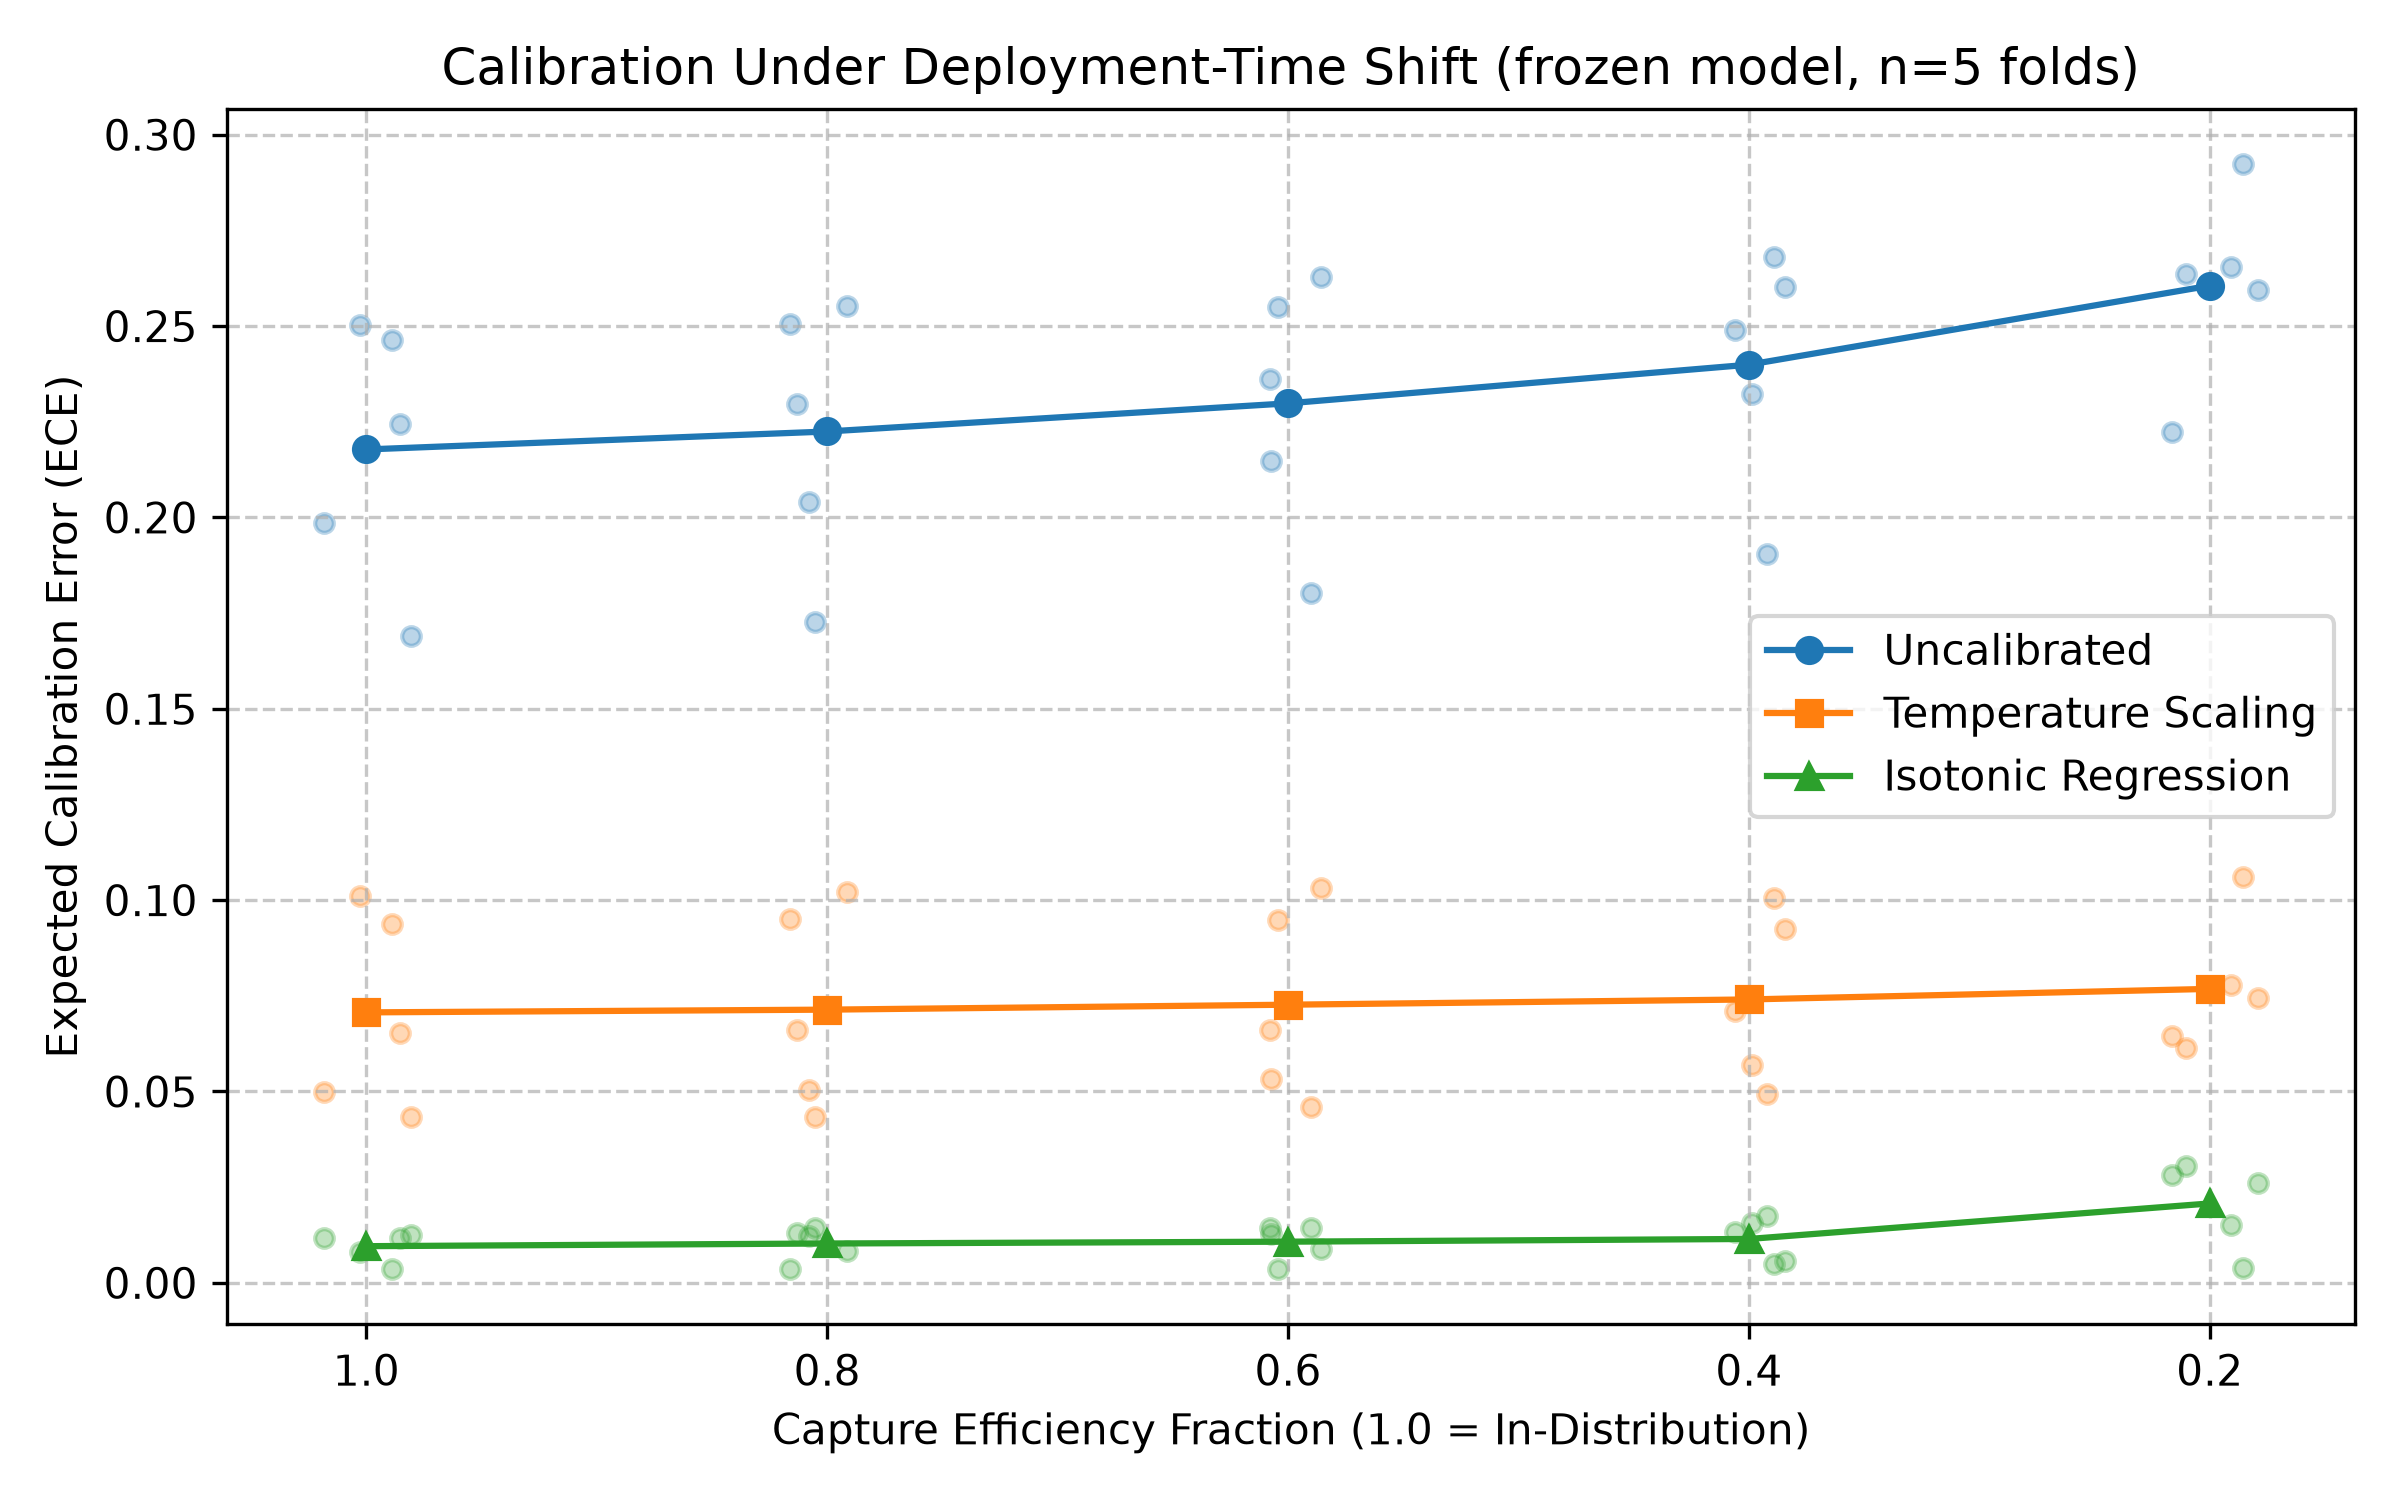
\includegraphics[width=0.8\linewidth]{figures/ece_degradation.png}
\caption{Calibration under deployment-time shift of simulated capture efficiencies, evaluated using a frozen DestVI model trained and calibrated exclusively on clean data (mean $\pm$ SEM across $n=5$ computational folds). Isotonic Regression's advantage over Temperature Scaling narrows as shift severity increases.}
\label{fig:ece}
\end{figure}

\subsection{Methodological Contribution: Isotonic Overfitting}
To formally test the hypothesis that Isotonic Regression overfits to the clean calibration split, we performed a controlled recalibration sweep. We generated a completely held-out calibration split subjected to the exact same deployment-time shift (80\% dropout) as the test set, and refit both calibrators. When Isotonic Regression was granted access to this shifted calibration split, its ECE improved significantly from $0.028$ down to $0.012$. This provides strong evidence for the hypothesis that its severe degradation under shift is attributable to overfitting to the source distribution's confidence profile. In contrast, Temperature Scaling's single-parameter simplicity provided inherent regularization, demonstrating no meaningful difference between clean-fit ($ECE~0.069$) and shift-fit ($ECE~0.069$) performance.

\subsection{Calibration Degradation Across Diverse Technical Shifts}
To confirm that Isotonic Regression's vulnerability to distribution shift is not an isolated artifact of capture efficiency dropout, we expanded our synthetic evaluation to encompass ambient Poisson noise injection. Consistent with our capture efficiency findings, Temperature Scaling demonstrated superior relative stability: under severe noise injection, Isotonic Regression's ECE degraded from $0.010$ to $0.016$, while Temperature Scaling actually showed a slight ECE improvement from $0.067$ to $0.054$. This artificial improvement occurs because severe ambient Poisson noise drives predictions closer to a high-entropy uniform distribution. Since the model was overconfident at baseline, this flattening naturally lowers the confidence and artificially reduces ECE, highlighting the metric's sensitivity to the underlying entropy of the shift. Nevertheless, this supports the notion that the single-parameter regularization of Temperature Scaling provides critical stability under diverse, unpredictable technical domain shifts. In terms of Compositional RMSE, baseline error was $0.0987$, degrading moderately under 80\% dropout ($0.1056$) and improving under severe Poisson noise ($0.0894$), further capturing these entropic shifts.

\subsection{Multi-Model Comparison: cell2location}
To evaluate whether these calibration vulnerabilities generalize to other prominent spatial architectures, we extended our benchmark pipeline to evaluate \texttt{cell2location}. Unlike the amortized inference in DestVI, \texttt{cell2location} optimizes parameters on a per-spot basis. Under five seeded repeated holdout replicates, \texttt{cell2location} exhibited severe innate miscalibration, reaching an uncalibrated ECE of $0.396 \pm 0.005$ on clean data. This severe baseline miscalibration is consistent with known behaviors in the spatial deconvolution literature, where \texttt{cell2location}'s un-amortized Bayesian hierarchical model has been observed to confidently overrepresent dominant cell types if the single-cell reference is not perfectly matched to the target tissue \citep{kleshchevnikov2022cell2location, sun2024tissue}. Crucially, Temperature Scaling failed to correct this model within the standard bounded optimization space. Because the per-spot optimization causes the un-calibrated posteriors to become severely skewed under shift, the single scalar parameter of Temperature Scaling (bounded to $T \in [0.5, 3.0]$) is structurally insufficiently expressive to flatten the distribution without collapsing it entirely to uniform, leaving the calibrated ECE as high as $0.378 \pm 0.006$ under 80\% capture dropout. To verify this, we note that the classification AUROC degraded severely from clean to shifted conditions (from $0.92$ down to $0.76$), and Temperature Scaling was permanently pinned to the $T=3.0$ maximum boundary. In stark contrast, Isotonic Regression's non-parametric mapping can project an entire dense block of high confidences to a flat empirical base rate (acting as a step function), successfully recalibrating the model to an ECE of $0.047 \pm 0.005$ (clean) and $0.050 \pm 0.006$ (shifted). This visually resulted in a sharp step-wise isotonic fitted curve (Appendix C). This demonstrates that for non-amortized models whose confidence distributions become severely skewed, Temperature Scaling is inadequate and Isotonic Regression is preferable under the conditions tested (Figure \ref{fig:multimodel}). We emphasize that this is a comparison of one specific architecture pair (DestVI vs.\ \texttt{cell2location}), not a universal claim about all amortized versus per-spot models.

\begin{figure}[htbp]
    \centering
    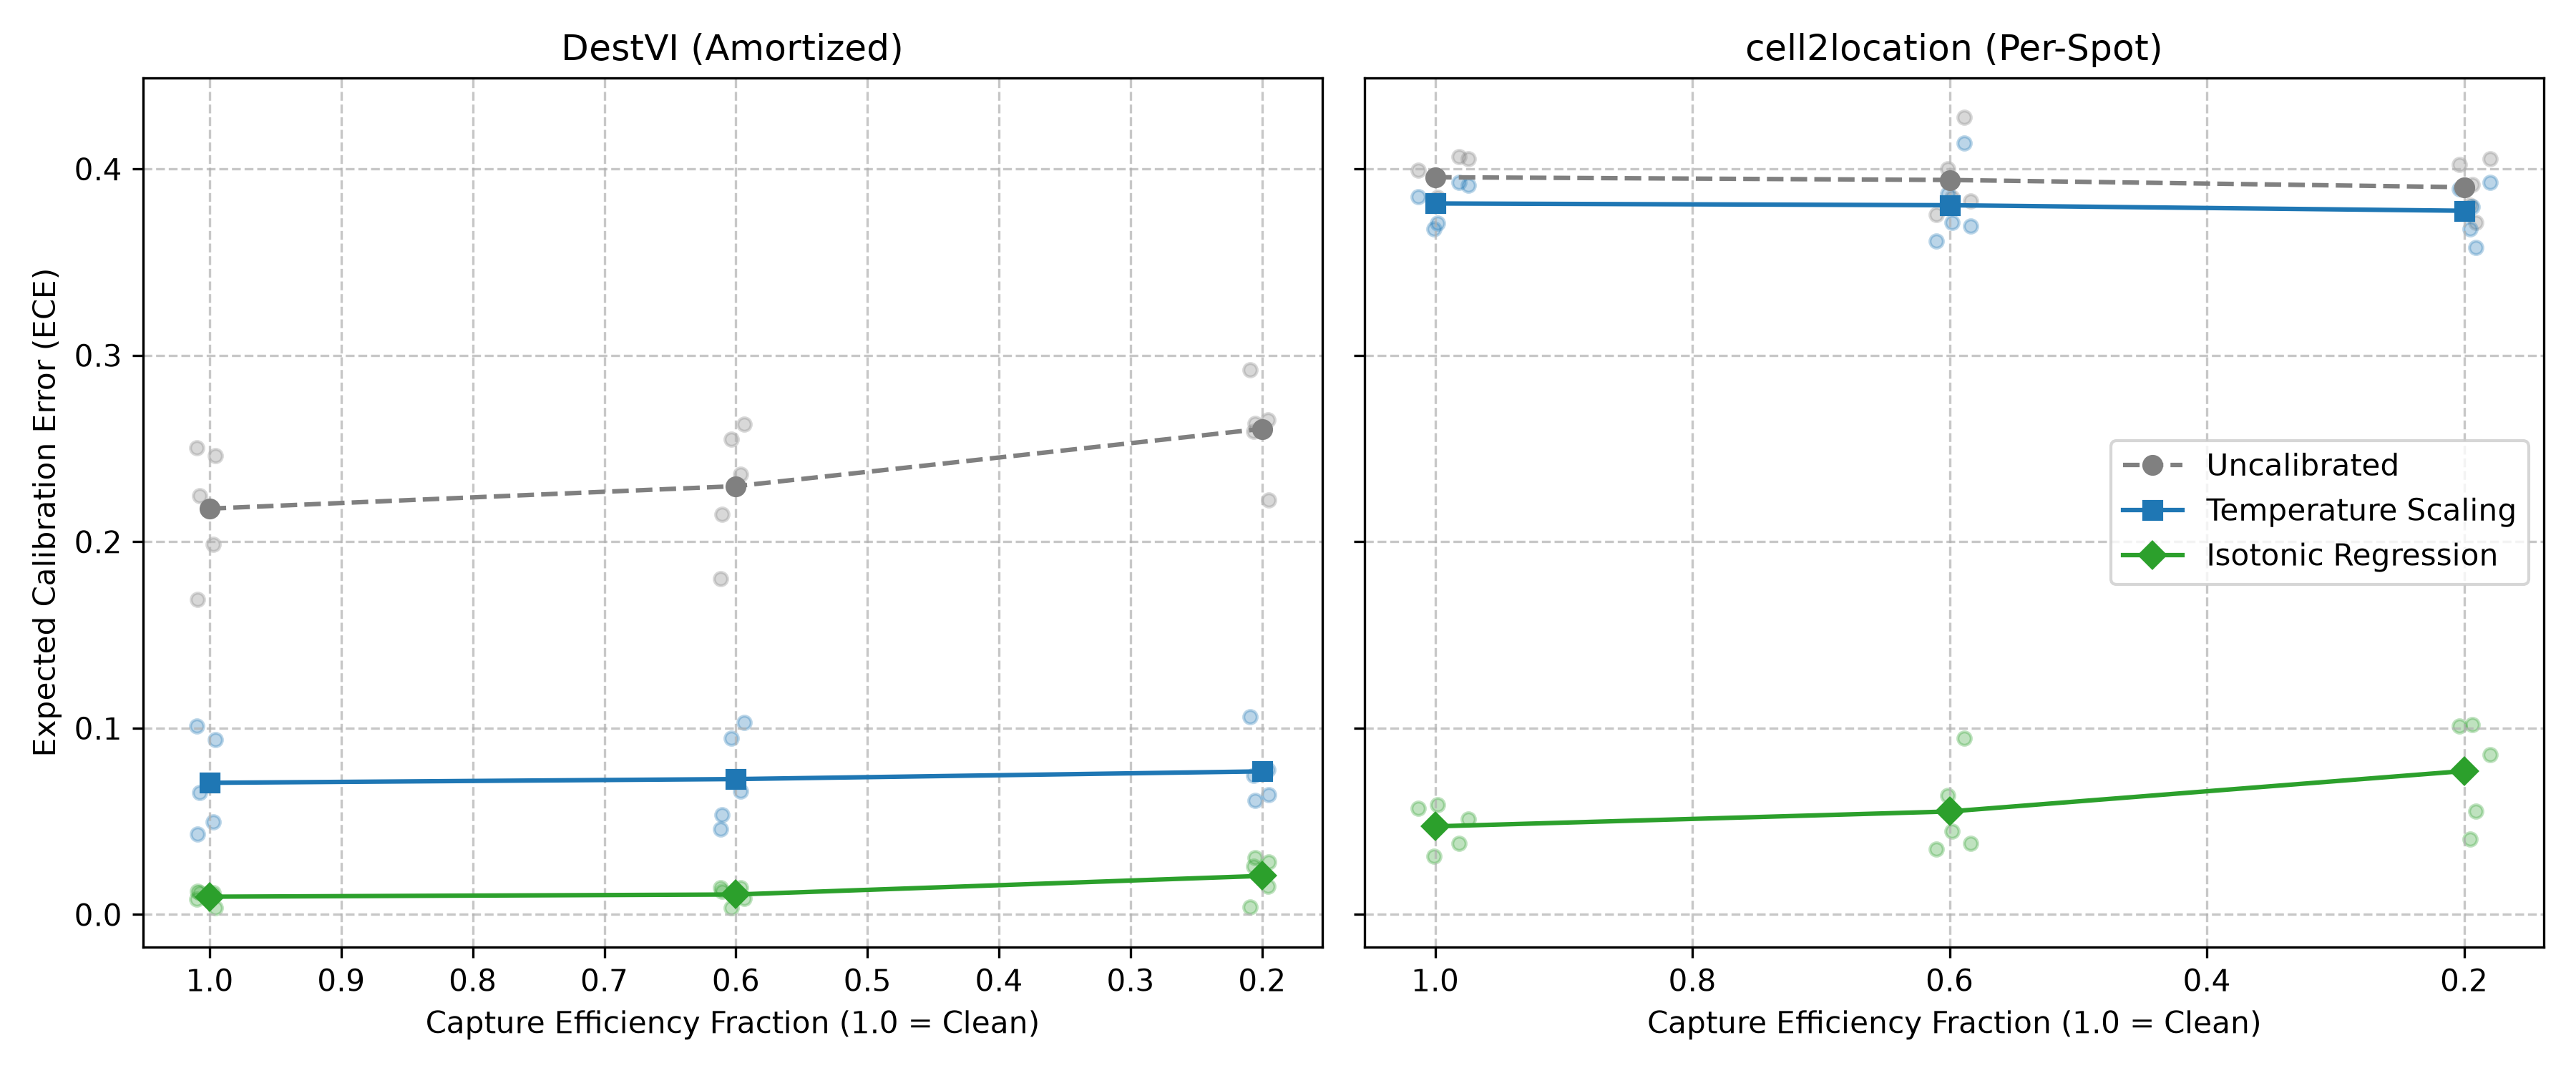
\includegraphics[width=0.7\linewidth]{figures/multimodel_ece.png}
    \caption{Multi-Model calibration comparison under capture efficiency shift (mean $\pm$ SEM across $n=5$ computational folds). While Temperature Scaling robustly corrects DestVI, it only partially corrects \texttt{cell2location}, leaving a substantial calibration gap.}
    \label{fig:multimodel}
\end{figure}

\subsection{Taxonomic Granularity Ablation}
Our primary analyses were conducted at the \textit{subclass} granularity ($k=23$ cell types). In spatial transcriptomics, the taxonomy dictates the complexity of the marginal confidence density. At $k=23$ fine-grained classes, the marginals are sparse, restricting the fitted isotonic map to a limited region of confidence support ($0.04\text{--}0.63$). Because sparse marginals leave large stretches of the fitted map estimated from few calibration points, the redistribution of mass under shift lands predictions in these poorly-estimated regions, destroying calibration. In contrast, at a $k=4$ coarse taxonomic resolution, the marginal density is broad and dense ($0.33\text{--}0.93$), providing comprehensive support coverage across the probability range (Figure \ref{fig:knots}). 

\begin{figure}[htbp]
    \centering
    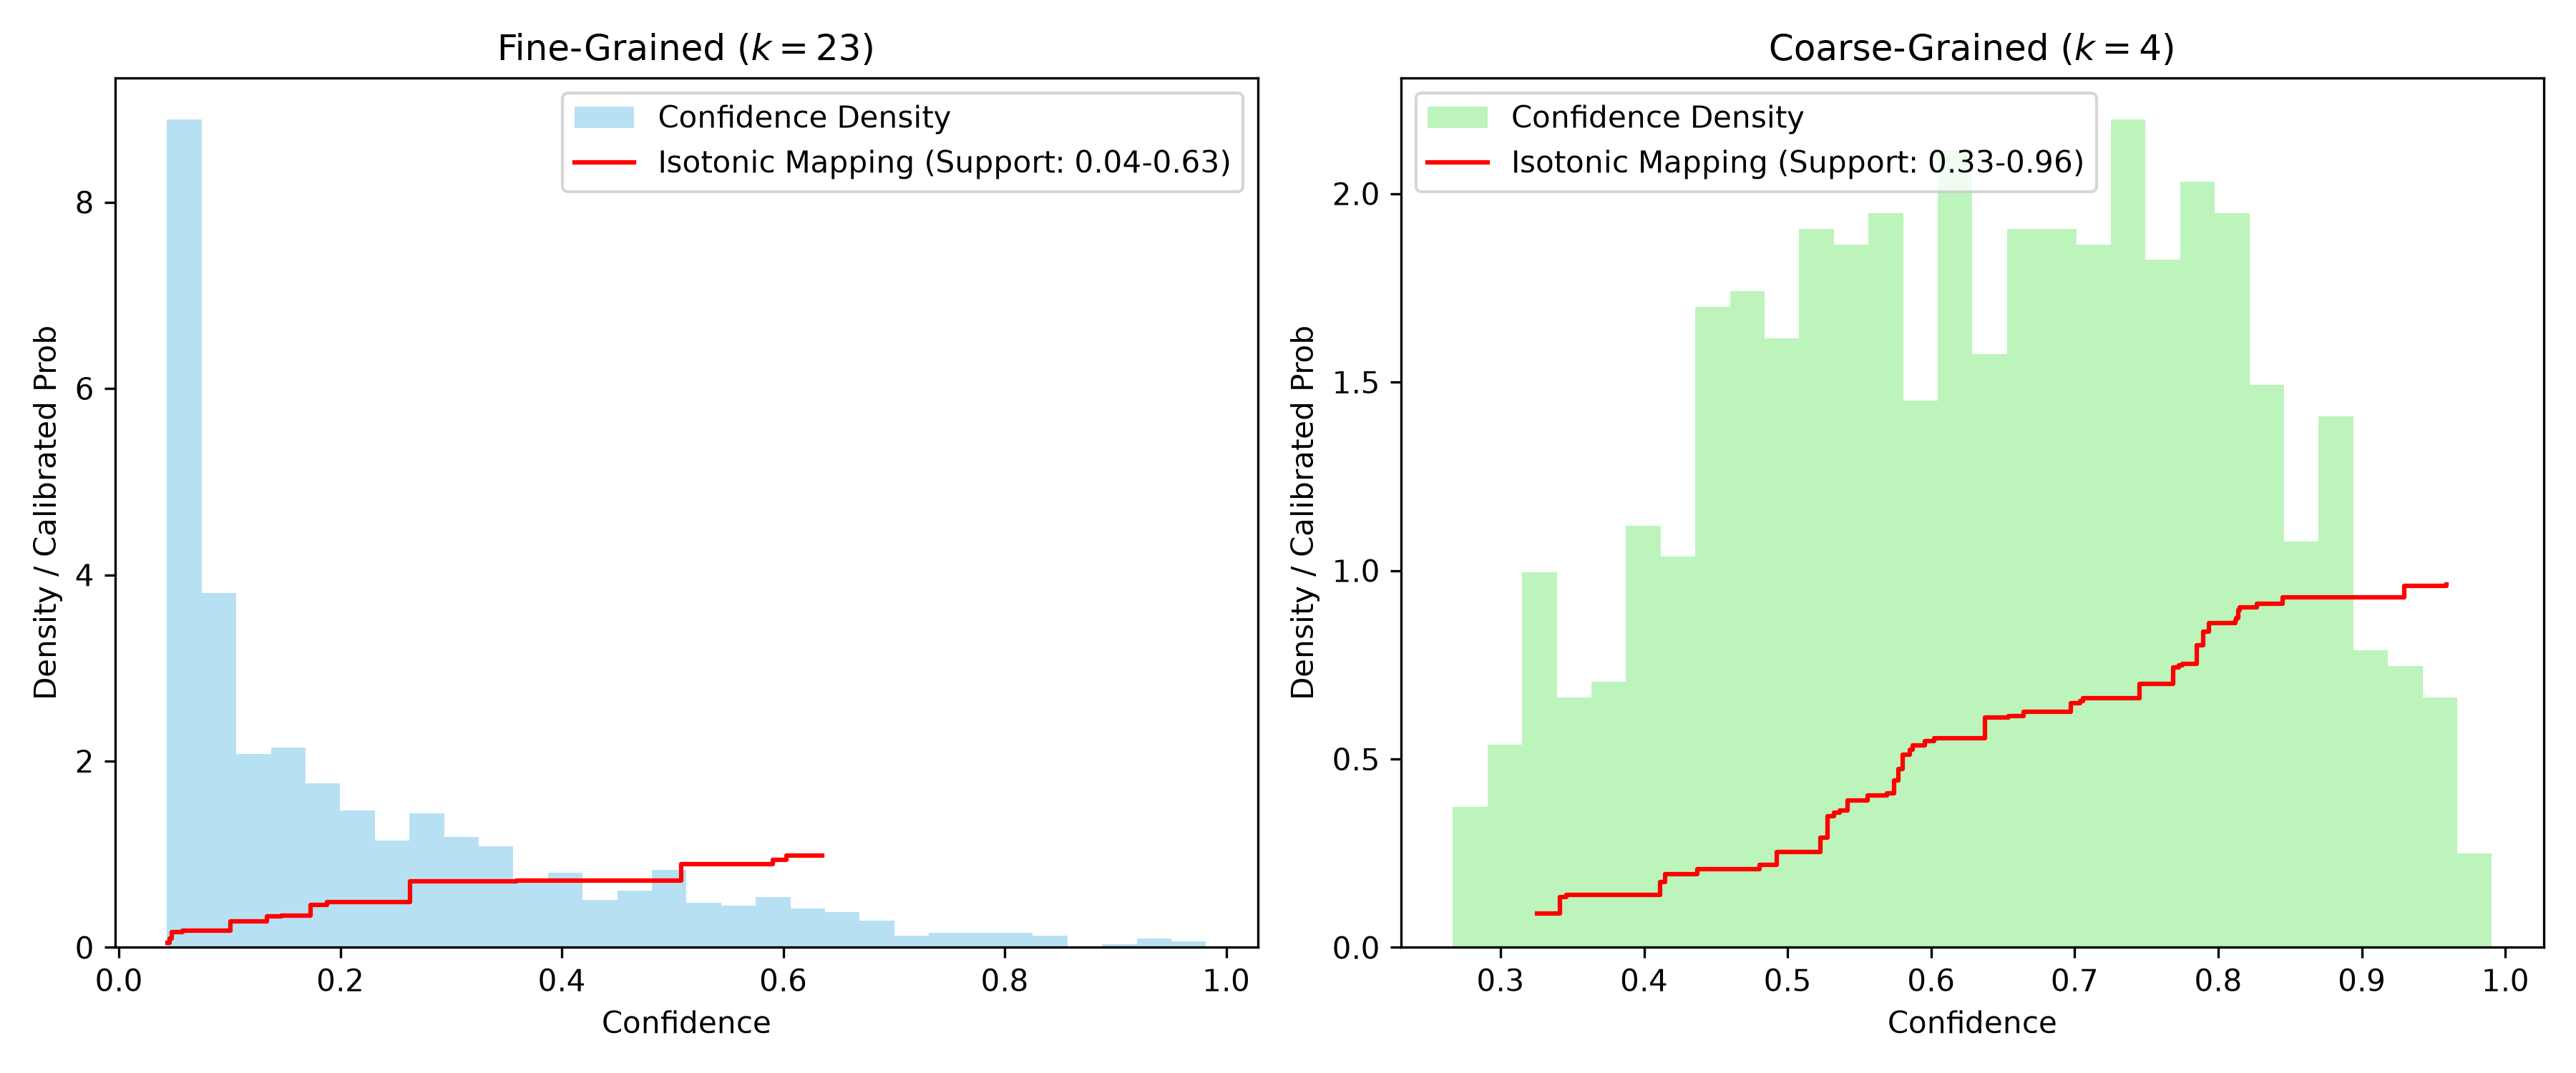
\includegraphics[width=0.7\linewidth]{figures/granularity_knots.png}
    \caption{Confidence density and Isotonic Regression mappings across taxonomic granularities. Fine granularity ($k=23$) restricts the fitted mapping to a narrow region of support, making it fragile out-of-distribution. Coarse taxonomic granularity ($k=4$) generates broad, dense marginal confidences, providing comprehensive support coverage across the full probability range.}
    \label{fig:knots}
\end{figure}

On the clean synthetic cortex mapped to coarse $k=4$ groupings, the DestVI baseline ECE was $0.571 \pm 0.003$. Temperature Scaling was catastrophically rigid: attempting to calibrate the $k=4$ posteriors pushed the parameter to the absolute search boundary ($T=3.0$), resulting in a completely flat ECE-vs-T curve that strictly degraded the calibration from the baseline ($0.582 \pm 0.002$). Conversely, Isotonic Regression successfully achieved an ECE of $0.011 \pm 0.001$, and critically, did not suffer relative degradation under $80\%$ dropout ($0.012 \pm 0.001$). However, we note that these ECE values ($0.011$) fall below the theoretical expected noise floor ($0.041$) for this coarse task, indicating that while Isotonic Regression avoids severe out-of-distribution relative degradation here, its absolute ECE magnitude remains artificially deflated by binning artifacts. At $k=4$, the dense marginals intrinsically regulate the non-parametric estimator, ensuring the fitted map is robustly estimated across nearly the full confidence range so that shifted predictions are mapped accurately. This is consistent with reports that method performance is highly sensitive to extreme class imbalances \citep{sang2024spotless}. 

To determine if the architectural and granularity vulnerabilities interact, we evaluated \texttt{cell2location} at this same coarse class level. Consistent with our architectural findings, Temperature Scaling failed to fully correct the baseline miscalibration (ECE $0.591 \pm 0.002$ uncalibrated vs.\ $0.534 \pm 0.001$ calibrated). However, because the coarse granularity provides dense marginals, Isotonic Regression successfully rescued the model without suffering the severe relative degradation seen in fine-grained tasks, retaining an excellent ECE of $0.026 \pm 0.003$ (clean) and $0.034 \pm 0.005$ (shifted at 80\% dropout). This asymmetry highlights that while Temperature Scaling under-corrects \texttt{cell2location} at coarse granularity, it actually backfires and degrades DestVI. This is consistent with Isotonic Regression being the stronger choice when non-amortized optimization and coarse taxonomic resolution coincide.

\subsection{Synthetic Verification of Overfitting}
\label{sec:synthetic}
To rule out the possibility that Temperature Scaling's stability is simply an artifact of the shift magnitude, we designed a synthetic experiment to cleanly isolate marginal shift from true conditional miscalibration. We generated synthetic probabilities using a non-linear power mapping (squaring the true proportions to induce severe overconfidence). Importantly, this means that the underlying true miscalibration map is not a scalar temperature scaling function. We then sampled ground truth labels from these underlying proportions, creating a perfectly defined calibration manifold with no finite-sample model training artifacts. We then simulated a deployment-time shift solely by changing the Dirichlet parameters generating the marginal class distribution $\alpha$, without altering the underlying calibration mapping.

Isotonic Regression successfully minimized ECE on the clean test data (achieving $0.013$ compared to the uncalibrated $0.162$). However, despite the true calibration mapping remaining entirely unchanged between the environments, Isotonic Regression's ECE on the shifted test data degraded severely to $0.062$. This confirms that Isotonic Regression overfits to the empirical marginal density of the clean data, and any shift in class prevalence or confidence density corrupts its non-parametric mapping. Conversely, Temperature Scaling (despite being structurally mis-specified for the power mapping) proved remarkably robust to the marginal shift, maintaining excellent calibration across both environments ($0.011$ clean vs.\ $0.008$ shifted). This cleanly demonstrates that Temperature Scaling's single-parameter formulation protects it against marginal density overfitting, rendering it substantially more robust to distribution shift than non-parametric alternatives, even when it is structurally mis-specified for the true confidence distribution.

\subsection{Secondary Robustness Check on Authentic Spatial Tissue}
To ensure our findings are not artifacts of the synthetic environment, we qualitatively applied the uncalibrated model and Temperature Scaling to real spatial datasets (a Visium lymph node and mouse cortex). Temperature Scaling ($T=2.0$) derived from synthetic sweeps effectively softened the uncalibrated, near-deterministic cell-type assignments into biologically plausible mixture profiles. This suggests that the calibration dynamics identified in controlled environments generalize to correct overconfidence in authentic deployment settings, even where exact single-cell ground truth is unavailable for quantitative evaluation.

\subsection{Cross-Platform Generalization and Biological Misspecification}
While synthetic shifts isolate technical noise, real-world deployment frequently involves cross-platform domain shifts. We observed that spatial models are highly sensitive to biological misspecification; however, strictly harmonizing Slide-seqV2 spatial data with an anatomically matched DropViz single-cell reference allowed the model to generalize well across platforms, producing visually plausible spatial assignments without requiring post-hoc calibration. This underscores the necessity of validating calibration dynamics across multiple distinct biological systems.

\section{Limitations}
\label{sec:limitations}
We note several limitations. To ensure feasibility, models were trained for up to 200 epochs using early stopping on 50\% of available pseudo-spots. Furthermore, our synthetic evaluations rely on binomial dropout and Poisson noise on mouse cortex data, though offset by qualitative real-tissue checks. Future research should investigate inherently risk-calibrated architectures.

\section{Discussion and Conclusion}
\label{sec:conclusion}
Confidence in spatial transcriptomics deconvolution is substantially miscalibrated at baseline and degrades under deployment-time shift. Rather than identifying a universally superior calibrator, our results suggest that calibration robustness is highly conditional. For fine-grained taxonomic classification, Isotonic Regression retains an absolute numerical advantage over Temperature Scaling across tested shifts, but its steep relative degradation trajectory poses a severe stability concern. A controlled synthetic experiment (Section 5.6) isolates this vulnerability, demonstrating that Isotonic Regression is highly sensitive to marginal density shifts even when the underlying true miscalibration map is constant. Overfitting to the source marginal produces a narrow support coverage for the fitted mapping, meaning that any shift in class prevalence or confidence density pushes predictions out-of-distribution where they are clipped and miscalibrated. Conversely, for coarse-grained classification, broad support coverage prevents Isotonic density-shift degradation, while Temperature Scaling becomes overly restrictive, degrading DestVI outright and only partially correcting \texttt{cell2location}. Furthermore, DestVI and cell2location exhibit markedly different calibration-transfer behavior in our experiments: while Temperature Scaling rescues amortized models (DestVI), it cannot rescue models with un-amortized per-spot posteriors that become severely skewed under shift (\texttt{cell2location}), which instead require the more expressive, non-parametric flattening of Isotonic Regression. Accounting for both taxonomic resolution and model architecture when selecting calibration strategies is therefore essential for deploying reliable spatial transcriptomics pipelines.

\subsubsection*{Broader Impact Statement}
This foundational benchmarking work characterizes model calibration failure modes in spatial transcriptomics. Miscalibrated models pose tangible risks if integrated blindly into discovery pipelines, potentially giving false reassurance under technical shifts and skewing downstream analysis. Our results demonstrate that calibration efficacy depends heavily on taxonomic granularity and computational architecture. Relying on universal calibration heuristics could systematically bias biological discovery.

\bibliography{ref}

\appendix
\section{Reproducibility Details}
\label{app:reproducibility}
To facilitate full reproducibility of our empirical results, we detail the core hyperparameter and benchmarking configurations below:
\begin{itemize}
    \item \textbf{Data Generation:} The 5-fold cross-validation pipeline was seeded sequentially ($42$ to $46$) to generate distinct pseudo-spot datasets per fold. Clean pseudo-spots ($N=2000$ per replicate) were generated using 10 cells per spot from the held-out source-cell pools.
    \item \textbf{Model Training:} DestVI and CondSCVI models were trained with early stopping for up to 200 epochs using default learning rates. \texttt{cell2location} reference signatures were trained for up to 200 epochs, and per-spot spatial mapping was trained for up to 200 epochs with \texttt{detection\_alpha=20}.
    \item \textbf{Metrics:} Expected Calibration Error (ECE) was computed using the \texttt{netcal.metrics.ECE} implementation with \texttt{bins=10}. Continuous Brier Scores were similarly computed across the full probability manifolds as $\text{BS} = \frac{1}{N} \sum_{i=1}^{N} \sum_{c=1}^{k} (f_{i,c} - o_{i,c})^2$.
    \item \textbf{Calibration:} Temperature Scaling applied to the compositional outputs is mathematically defined as scaling the log-probabilities (with $\epsilon=10^{-7}$ for numerical stability) and renormalizing via softmax: $p'_i = \frac{\exp(\log(p_i + \epsilon) / T)}{\sum_j \exp(\log(p_j + \epsilon) / T)}$. It was optimized over the search space $T \in [0.5, 3.0]$ with 50 discrete steps to minimize ECE on the calibration split. Isotonic Regression was fit using the \texttt{sklearn.isotonic.IsotonicRegression} module with \texttt{out\_of\_bounds='clip'}, mapping the maximum predicted proportion to empirical correctness.
\end{itemize}

\section{Additional Calibration Metrics}
\label{app:additional_metrics}
Because ECE is highly sensitive to the number and width of confidence bins, we also evaluated calibrator performance using Adaptive-binning ECE (which partitions bins to contain an equal number of samples) and Negative Log-Likelihood (NLL). Due to space constraints, we summarize the findings here: while Isotonic Regression consistently minimized fixed-bin ECE across all shifts, both its fine-grained Adaptive-ECE (degrading from $0.015$ to $0.035$, compared to Temperature Scaling's stable $0.065$ to $0.068$) and coarse-grained Adaptive-ECE (degrading from $0.035$ to $0.037$) alongside NLL degraded significantly more rapidly than Temperature Scaling's under severe technical shift (e.g., Isotonic NLL increased from $1.51$ to $3.58$, while Temperature Scaling only increased from $1.52$ to $1.73$). This indicates that while Isotonic Regression successfully groups confidences to match aggregate empirical accuracy, it often degrades the likelihood of the true probability distribution, heavily suggesting binning-artifact overfitting. The parametric Beta[a=b] calibration model exhibited similar degradation trajectories to Isotonic Regression (Beta ECE degrading from $0.012$ to $0.027$), supporting our conclusion that the single-parameter robustness of Temperature Scaling provides unique regularization against distribution shift.

\section{\texttt{cell2location} Diagnostic Evaluation}
\label{app:c2l_diagnostic}
Unlike amortized models, \texttt{cell2location} fits a hierarchical Bayesian model per-spot, causing severe posterior skew under severe deployment-time shift (e.g., 80\% capture efficiency dropout). Under this shift, the classification AUROC collapsed significantly, producing a mass of high-confidence, low-accuracy predictions. Temperature Scaling was structurally unable to flatten this density (hitting the $T=3.0$ maximum boundary). In contrast, Isotonic Regression successfully learned a sharp step-function mapping, collapsing the dense block of overconfident predictions to the empirical base rate.

\section{ECE Noise Floor Simulation}
\label{app:noise_floor}
To compute the theoretical ECE noise floor for a perfectly calibrated model (Section 5.1), we simulated 5,000 empirical datasets. For each simulation, we sampled ground-truth test proportions from a uniform Dirichlet distribution across $k$ classes. To simulate $N=500$ perfectly calibrated spatial spots, we drew true labels directly from these spot-level true proportions. We then computed the maximum probability (confidence) and argmax class (prediction) for each spot, and evaluated the fixed-bin Expected Calibration Error (10 bins) against the sampled labels. Because the predictions are perfectly calibrated by definition, any non-zero ECE arises strictly from finite-sample binning noise. This yielded a mean expected noise floor of $0.021 \pm 0.010$ for $k=23$, and $0.041 \pm 0.013$ for $k=4$.

\end{document}
